\documentclass[a4j]{jarticle}
\usepackage{amsmath}
\usepackage{ascmac}
\usepackage{amssymb}
\usepackage{enumerate}
\usepackage{multicol}
\usepackage{framed}
\usepackage{fancyhdr}
\usepackage{latexsym}
\usepackage{indent}
\usepackage{cases}
\usepackage[dvips]{graphicx}
\allowdisplaybreaks
\pagestyle{fancy}
\lhead{}
\chead{}
\rhead{東京大学前期$1968$年$1$番}
\begin{document}
%分数関係


\def\tfrac#1#2{{\textstyle\frac{#1}{#2}}} %数式中で文中表示の分数を使う時


%Σ関係

\def\dsum#1#2{{\displaystyle\sum_{#1}^{#2}}} %文中で数式表示のΣを使う時


%ベクトル関係


\def\vector#1{\overrightarrow{#1}}  %ベクトルを表現したいとき(aベクトルを表現するときは\ver
\def\norm#1{|\overrightarrow{#1}|} %ベクトルの絶対値
\def\vtwo#1#2{ \left(%
      \begin{array}{c}%
      #1 \\%
      #2 \\%
      \end{array}%
      \right) }                        %2次元ベクトル成分表示
      
      \def\vthree#1#2#3{ \left(
      \begin{array}{c}
      #1 \\
      #2 \\
      #3 \\
      \end{array}
      \right) }                        %3次元ベクトル成分表示



%数列関係


\def\an#1{\verb|{|$#1$\verb|}|}


%極限関係

\def\limit#1#2{\stackrel{#1 \to #2}{\longrightarrow}}   %等式変形からの極限
\def\dlim#1#2{{\displaystyle \lim_{#1\to#2}}} %文中で数式表示の極限を使う



%積分関係

\def\dint#1#2{{\displaystyle \int_{#1}^{#2}}} %文中で数式表示の積分を使う時

\def\ne{\nearrow}
\def\se{\searrow}
\def\nw{\nwarrow}
\def\ne{\nearrow}


%便利なやつ

\def\case#1#2{%
 \[\left\{%
 \begin{array}{l}%
 #1 \\%
 #2%
 \end{array}%
 \right.\] }                           %場合分け
 
\def\1{$\cos\theta=c$,$\sin\theta=s$とおく.}  %cs表示を与える前書きシータ
\def\2{$\cos t=c$,$\sin t=s$とおく.}     %cs表示を与える前書きt
\def\3{$\cos x=c$,$\sin x=s$とおく.}                %cs表示を与える前書きx

\def\fig#1#2#3 {%
\begin{wrapfigure}[#1]{r}{#2 zw}%
\vspace*{-1zh}%
\input{#3}%
\end{wrapfigure} }           %絵の挿入


\def\a{\alpha}   %ギリシャ文字
\def\b{\beta}
\def\g{\gamma}

%問題番号のためのマクロ

\newcounter{nombre} %必須
\renewcommand{\thenombre}{\arabic{nombre}} %任意
\setcounter{nombre}{2} %任意
\newcounter{nombresub}[nombre] %親子関係を定義
\renewcommand{\thenombresub}{\arabic{nombresub}} %任意
\setcounter{nombresub}{0} %任意
\newcommand{\prob}[1][]{\refstepcounter{nombre}#1[問題 \thenombre]}
\newcommand{\probsub}[1][]{\refstepcounter{nombresub}#1(\thenombresub)}


%1-1みたいなカウンタ(todaiとtodaia)
\newcounter{todai}
\setcounter{todai}{0}
\newcounter{todaisub}[todai] 
\setcounter{todaisub}{0} 
\newcommand{\todai}[1][]{\refstepcounter{todai}#1 \thetodai-\thetodaisub}
\newcommand{\todaib}[1][]{\refstepcounter{todai}#1\refstepcounter{todaisub}#1 {\bf [問題 \thetodai.\thetodaisub]}}
\newcommand{\todaia}[1][]{\refstepcounter{todaisub}#1 {\bf [問題 \thetodai.\thetodaisub]}}


     \begin{oframed}
     平面上の点$(x,y)$で$x^2-5x<y<\cfrac{\pi}{5}\sin\left(\cfrac{\pi x}{5}\right)-\cfrac{3}{5}\sin^2\left(\cfrac{\pi x}{5}\right)$をみたす
     範囲が,直線$y=\a x$によって面積の等しい二つの部分に分けられるように,$\a$の値を求めよ.
     \end{oframed}

\setlength{\columnseprule}{0.4pt}
\begin{multicols}{2}
{\bf[解]} 簡単のため
     \begin{align*}
     \left\{
          \begin{array}{l}
          f(x)=x^2-5x \\
          g(x)=\cfrac{\pi}{5}\sin\left(\cfrac{\pi x}{5}\right)-\cfrac{3}{5}\sin^2\left(\cfrac{\pi x}{5}\right)
          \end{array}
     \right.
     \end{align*}
とおく.$0<x<5$では$f(x)<0$,$g(x)>0$である.
故にグラフの概形は下図.
\vspace{-3zh}
     \begin{center}
     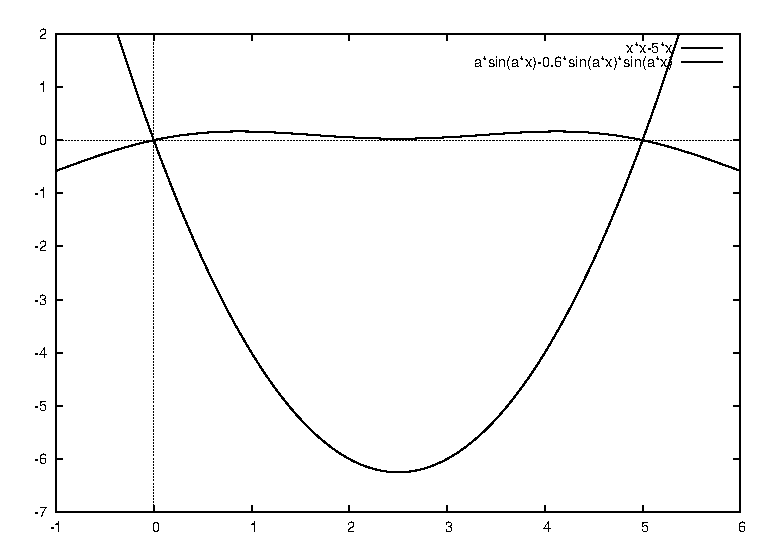
\includegraphics[width=6cm]{ut-68-1-a.eps}
     \end{center}
\vspace{2zh} 
これら二つのグラフの囲む面積$S$とすると,
     \begin{align}
     S=\int_0^5(g(x)-f(x))dx\label{1}
     \end{align}
である.各項計算すると,
     \begin{align*}
     &\cdot S_1=-\int_0^5f(x)dx=\frac{5^3}{6}=\frac{125}{6} \\
     &\cdot S_2=\int_0^5g(x)dx=\int_0^\pi\left(\sin t-\frac{3}{\pi}\sin^2t\right)dt \\
     &=\left[-\cos t-\frac{3}{2\pi}(t-2\sin 2t)\right]_0^\pi=2-\frac{3}{2}=\frac{1}{2}
     \end{align*}
である.故に\eqref{1}に代入して
     \begin{align}
     S=S_1+S_2=\frac{64}{3}\label{2}
     \end{align}
である.

また,$S_1>S_2$であるから,題意より,$\a<0$となることが必要で,このとき,$y=\a x$と$y=f(x)$が$0<x<5$に交点をひとつ持つ
.グラフの概形は右上図. 
    \begin{center}
     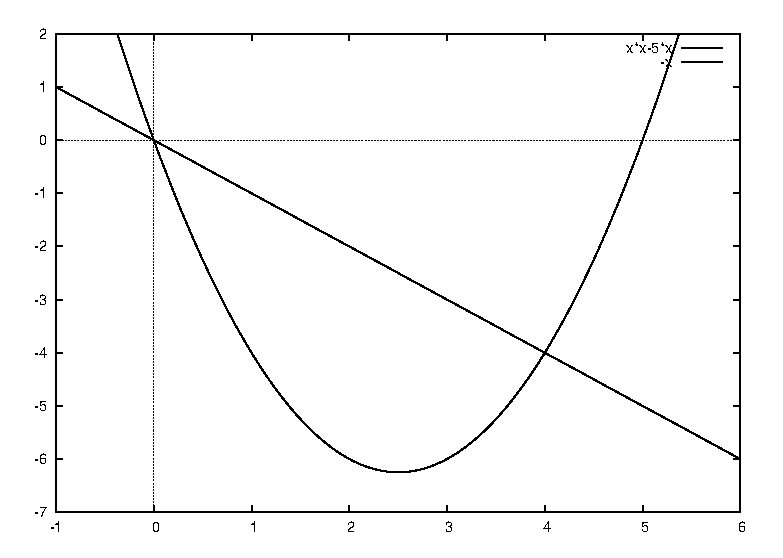
\includegraphics[width=6cm]{ut-68-1-b.eps}
     \end{center}
    
 \\
交点の$x$座標を$p$とおく.つまり
     \begin{align}
     &\begin{cases}
     0<p<5 \\
     \a p=p^2-5p
     \end{cases}\nonumber \\
     \Longleftrightarrow
     &\begin{cases}
     0<p<5 \\
     \a =p-5
     \end{cases}\label{3}
     \end{align}
とする.\eqref{2}に注意して,面積が等しい条件から
     \begin{align*}
     &\frac{1}{2}S=\int_0^p(\a x-f(x))dx \\
     \Longleftrightarrow &\frac{32}{3}=\frac{1}{6}p^3\\
     \Longleftrightarrow &p=4
     \end{align*}
である.これを\eqref{3}に代入して
     \[\a=-1\]
これは$\a<0$を満たし,十分.以上から,求める値は$\a=-1$である.$\cdots$(答)
\newpage
\end{multicols}
\end{document}